\documentclass[tikz,border=2pt]{standalone}
\usepackage{amsmath}
\usepackage{pgfplots}
\pgfplotsset{compat=1.18}
\usetikzlibrary{arrows.meta}
\begin{document}
% Left (Exercise 1.13): f(x)=x^2 on [0,3) with f(3)=10, a jump up at the endpoint 3; f is (strictly) convex.
% Right (Example 1.6, part of [-3,3] shown): f(x)=x^2 for x<=0, x-1 for x>0, f(0)=0, right limit -1;
% the chord from a=-1 to b=1/10 has height -8/11 at 0, below f(0)=0, so f is not convex.
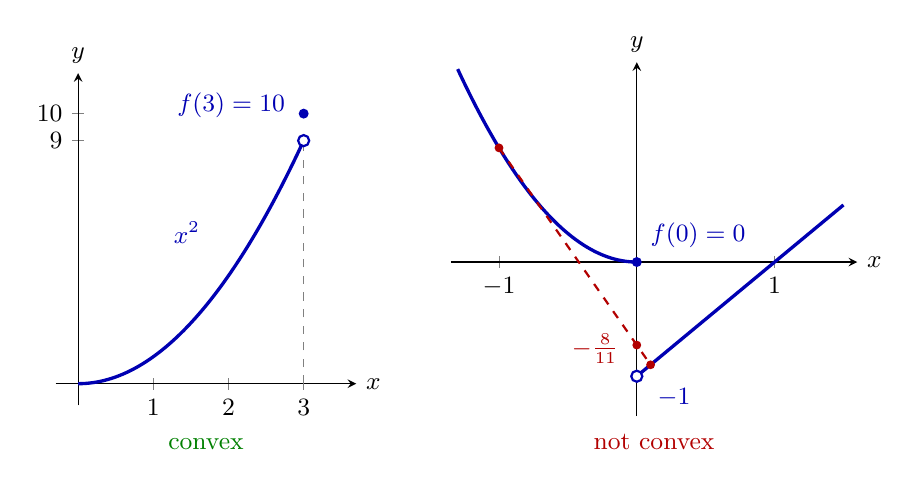
\begin{tikzpicture}[font=\small, >={Latex[length=2mm]}]
  \begin{axis}[
    name=left, axis lines=middle, xmin=-0.3, xmax=3.7, ymin=-0.8, ymax=11.5,
    xtick={1,2,3}, ytick={9,10},
    xlabel={$x$}, ylabel={$y$},
    xlabel style={anchor=west}, ylabel style={anchor=south},
    width=5.4cm, height=5.8cm, clip=false
    ]
    \addplot[blue!70!black, very thick, domain=0:2.97, samples=60] {x^2};
    \draw[gray, thin, dashed] (axis cs:3,0) -- (axis cs:3,9);
    \filldraw[fill=white, draw=blue!70!black, thick] (axis cs:3,9) circle (2pt);
    \fill[blue!70!black] (axis cs:3,10) circle (1.8pt);
    \node[blue!70!black, anchor=east] at (axis cs:2.88,10.3) {$f(3)=10$};
    \node[blue!70!black, anchor=east] at (axis cs:1.75,5.6) {$x^2$};
  \end{axis}
  \begin{axis}[
    name=right, at={(left.east)}, anchor=west, xshift=1.2cm,
    axis lines=middle, xmin=-1.35, xmax=1.6, ymin=-1.35, ymax=1.75,
    xtick={-1,1}, ytick=\empty,
    xlabel={$x$}, ylabel={$y$},
    xlabel style={anchor=west}, ylabel style={anchor=south},
    x=1.75cm, y=1.45cm, clip=false
    ]
    \addplot[blue!70!black, very thick, domain=-1.3:0, samples=60] {x^2};
    \addplot[blue!70!black, very thick, domain=0.03:1.5, samples=2] {x-1};
    \fill[blue!70!black] (axis cs:0,0) circle (1.8pt);
    \filldraw[fill=white, draw=blue!70!black, thick] (axis cs:0,-1) circle (2pt);
    \node[blue!70!black, anchor=south west] at (axis cs:0.03,0.04) {$f(0)=0$};
    \node[blue!70!black, anchor=north west] at (axis cs:0.08,-1.02) {$-1$};
    \draw[red!70!black, thick, dashed] (axis cs:-1,1) -- (axis cs:0.1,-0.9);
    \fill[red!70!black] (axis cs:-1,1) circle (1.6pt);
    \fill[red!70!black] (axis cs:0.1,-0.9) circle (1.6pt);
    \fill[red!70!black] (axis cs:0,-0.7273) circle (1.6pt);
    \node[red!70!black, anchor=east] at (axis cs:-0.06,-0.76) {$-\tfrac{8}{11}$};
  \end{axis}
  \node[green!50!black, anchor=north, text height=1.5ex, text depth=0.25ex, yshift=-2pt] at (left.south |- right.outer south) {convex};
  \node[red!70!black, anchor=north, text height=1.5ex, text depth=0.25ex, yshift=-2pt] at (right.south |- right.outer south) {not convex};
\end{tikzpicture}
\end{document}
